\section{Validation}

This section reviews the validation of immersed boundary methods.
The main goal of this validation is to determine the numerical error and the
numerical stability of a method.
Furthermore it is important to test if a  method supports the
the laws of conservation, in particular the conservation of mass.
In the first part of this section an introduction to different testcases
will be given. Three different test problem were chosen,
the poisseille flow, hagen-poiseuille flow and the taylor-couette system.
In the 2nd part the result for the different testcases will
be presented and discussed.

%In general it is necessary to obtain a good evaluation of the numerical truncation error,
% the numerical stability over longer periods of time
%and Grid convergence studys against theoretical and high-resolution numerical solutions
%will be performed and compared for the different IBMs.
%This part of the thesis the thesis deals with the numerical validation of the immersed
%boundary methods
%In order to ensure a correct numerical behavior of the introduced methods, a
%Multiple examples from simple to more complex testcases are introduced in this section.

\subsection{Laminar Poiseuille-Flow}

\begin{figure}[!bp]
  \begin{minipage}[c]{0.6\textwidth}
      \centering
        \resizebox{0.9 \textwidth}{!}{
       \import{gfx/immersed_boundary/poiseuille_flow//}{setup.pdf_tex}
      }
  \end{minipage}
  \begin{minipage}[c]{0.3\textwidth}
      \caption{Theoretical setup of the poiseuille-flow channel.
      \label{validation:setup_pf}
      }
  \end{minipage}
\end{figure}

The first testcases is the laminar poiseuille-flow, the theoretical setup is presented in Fig. \ref{validation:setup_pf}.
It consist of two infintiy long planes at $z=h_1$ and $z=h_2$ which are oriented
parallel to the xy-plane at a distance $\Delta h = h_2 - h_1$.
Numerically this is realized by using periodic boundaries in xy-direction and
No-Slip boundaries in z-direction.

The velocity profile results from a pressure gradient in x-direction, which is added into the naviers-stokes equation.
No other forces are present furthermore the flow will be independent of the y coordinate,
hence for the steady state $\partial v_x /\partial t = 0$ the non-dimensinoal equations of motion can be reduced to:

\begin{align}
\frac{\partial v_x}{\partial t} &= - \frac{\partial p}{\partial x}
 + \frac{1}{Re} \frac{\partial^2 v_x}{\partial z^2} = 0
\end{align}

with $Re = \nicefrac{V_{m}\Delta h}{\nu}$.
For the non-dimenzionalization we choose $r^* = r/\Delta h$, $v^*=V_(\text{m})/\Delta h$, $t^* = \frac{V_{\text{m}}}{\Delta h}$
and $p^* = p \rho V_{\text{max}}^2$

The equation can simply be integrated twice which yields the solution

\begin{align}
v_z &= \frac{1}{2}\frac{\partial p}{\partial x}z^2 + zc_1 + c_2
\end{align}

Using the NoSlip-boundary condition $v_x(h_1) = v_x(h_2) = 0$ and furthermore by defining
$A:=\frac{1}{2}\frac{\partial p}{\partial x} Re$ one obtains the additional conditions

\begin{align}
c_1 &= A\frac{h_1^2 -h_2^2}{h_2 - h_1} = -A(h_1+h_2)\\
c_2 &= A(h_1(h_1 + h_2) - h_1^2) = Ah_1h_2\\
\end{align}

The velocity is than given by the quadratic function

\begin{align}
v_x &= A(z^2 - z(h_1 + h_2) + h_1h_2)
\end{align}

The maximum velocity and postinon can be obtained by simple calculus

\begin{align}
z_{max} &= \frac{h_1+h_2}{2} \wedge v_{max} = A\left(h_1h_2 - \frac{(h_1 + h_2)^2}{4}\right)
\end{align}

Since $v_{max}$ has to be 1 by definition of the non-dimensionalzation we find

\begin{align}
\frac{\partial p}{\partial x} &= \frac{2}{Re}\frac{1}{\left(h_1h_2 - \frac{(h_1+h_2)^2}{4} \right)}
\end{align}

as a necessary condition for the pressure gradient.\\

\clearpage


\section{Simulations}

-Following conventions dx, N etc


\subsection{Poiseuille Flow}

The poiseuille-flow problem  is used in particular as a first validation testcase
for the Volume-Penalization and Direct-Forcing methods.

\subsubsection{Test of the Default Setup}

The purpose of the first simulation is the test of the default
implementation of the algorithm, without the use of immersed boundaries.
For this test case this is still possible since the geometry is non-curved
and parallel to the cartesian grid.
A grid convergence test was performed with the main simulation parameters are given by

\begin{center}
\vspace*{0.7ex}
\begin{tabular}{c|c|c|c|c|c|c }
 $ N  $                   & $\Delta t$ & $\Delta x$            & $\Rey$  & $c^2$   & $l_x, l_y, l_z$ & $T_{end}$\\
\hline
 $[8, 256], \Delta N = 8 $& $10^{-4}$ & $\nicefrac{1}{N - 1}$ & 500     & $500$   & (1, 1, 1)       & 10\\
\end{tabular}
\vspace*{0.7ex}
\end{center}

For all resolutions the simulations were performed for finite difference
schemes of 2nd and 4th order.

\subsubsection{Test of the Volume Penalization Method}

%With the given theoretical solution, the next objective is the comparison
%to the default implementation, the volume penalization method and the direct forcing method.
%Since we have a flow parallel to the grid  it does not make sence to compare it to the interpolation methods
%For the comparision with a theoretical solution it is necessary to ensure that
% the surface grid points match with the total height $h$ of the channel.

For the immersed boundary methdos the upper- and lower boundaries of the channel are realized by the masking function.
\begin{align}
H(x, y, z) = \begin{cases}
                    0, & \text{for \  }  h_1 \leq z \leq h_2 \\
                    1, & \text{else}.
             \end{cases}
\end{align}

For the volume penalization method we furthermore obtain a
The non-dimensionalized damping force  given by

\begin{align}
    \vec{f} = \frac{H}{J}v
\end{align}

where $J = \nicefrac{V_{m}}{\eta}$.

\clearpage

A first test is to investigate the error of the velocity profile, with a variation of the Reynolds-number and the damping rate $J$.
The total simulation domain is set to the height $l_z=2$ with $h_1=0.25$ and $h_2=0.75$.
A simulation series was performed with the main simulation parameters given by


\begin{center}
\vspace*{0.7ex}
\begin{tabular}{c|c|c|c|c|c|c|c }
 $ \Rey  $                      & $J$ &  $\Delta t$ & $\Delta x$            & $\Rey$  & $c^2$   & $l_x, l_y, l_z$ & $T_{end}$\\
\hline
 $[100, 500], \Delta \Rey = 25 $& $[10^{-5}, 5\cdot10^{-1}]  $ &  $10^{-4}$ & $\nicefrac{1}{N - 1}$ & 500     & $500$   & (1, 2, 0.25)  & 10\\
\end{tabular}
\vspace*{0.7ex}
\end{center}

The damping force was divided by 2 or 5 for n times.
To make sure that the channel width is equal to $\Delta h = 1$, the total height was set to $l_z\approx2.01587$.
This furthermore ensures that the grid points overlap exactly
with the masking function at $h_1$ and $h_2$.
This test was performaed for 2nd order (oder 4th order error explain)

As a second test a grid convergence study was carried out, with a constant Reynolds number and $\nu \in [1-23]$.
The resolution was varied between $N\in [4, 400]$ with $\Delta N = 4$, 2nd and 4th order schemes were tested.

\begin{center}
\vspace*{0.7ex}
\begin{tabular}{c|c|c|c|c|c|c|c }
 $ \Rey  $                      & $J$ &  $\Delta t$ & $\Delta x$            & $\Rey$  & $c^2$   & $l_x, l_y, l_z$ & $T_{end}$\\
\hline
 $[100, 500], \Delta \Rey = 25 $& $[10^{-5}, 5\cdot10^{-1}]  $ &  $10^{-4}$ & $\nicefrac{1}{N - 1}$ & 500     & $500$   & (1, 2, 0.25)  & 10\\
\end{tabular}
\vspace*{0.7ex}
\end{center}

\subsection{Test of the Direct Forcing Method}

Since the direct forcing method does not depend on a damping parameter it is sufficient enough
to carry out a grid convergence study
The simulation parameter arg given by

\begin{center}
\vspace*{0.7ex}
\begin{tabular}{c|c|c|c|c|c|c|c }
 $ \Rey  $                      & $J$ &  $\Delta t$ & $\Delta x$            & $\Rey$  & $c^2$   & $l_x, l_y, l_z$ & $T_{end}$\\
\hline
 $[100, 500], \Delta \Rey = 25 $& $[10^{-5}, 5\cdot10^{-1}]  $ &  $10^{-4}$ & $\nicefrac{1}{N - 1}$ & 500     & $500$   & (1, 2, 0.25)  & 10\\
\end{tabular}
\vspace*{0.7ex}
\end{center}

2nd and 4th order finite difference schemes were tested.

\clearpage

\section{Results}
\subsection{Poiseuille Flow}
\subsubsection{Default seutp}

The results of the grid convergence study are shown in figure \ref{fig:ema1}.
The double logarithmic axis shows the dependency of the computed relative $l_2$-error norm
with respect to the grid resolution.

On this scale, the 4th order finite differnce schemes has a linear decreasing error.
For the smallest resolution $N=8$ the error is of order $10^{-3}$,
in contrast to the highest resolution $N=256$, with an error of order $10^{-6}$
A convergence rate of the error  was computed by linear interpolation in the log-log space,
the results is about -2.257.
Hence, it can be said that the accuracy of the method is of 2nd order for this testcase,
which is is in contradiction with the theory.

The error of the second order finite difference scheme is of the order $10^{-8}$.
The value is approximately constant and not depend of the grid resolution.


\begin{figure}[!bp]
    \centering
    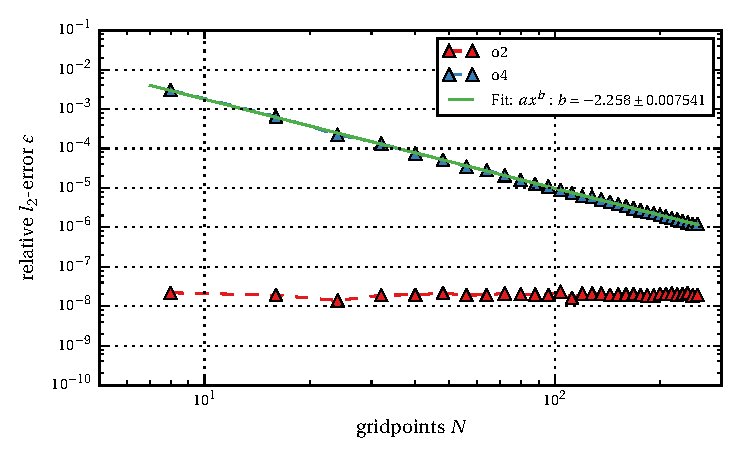
\includegraphics{gfx/immersed_boundary/poiseuille_flow/1_default/relative_l2error.pdf}
    \caption{Relative $l_2$-error for 2nd and 4th order finite difference schemes of the default algorithm without the use of an immersed boundary.\label{fig:ema1}}
\end{figure}

\clearpage


\subsubsection{Test of the Volume Penalization Method}

The first simulation was  a parameter study with variable Reynolds number $Re$ and damping rate $J$.
A first impression of the influence of the damping rate $J$ , is given by the velocity profiles of the numerical solution.
This is exemplarily shown in figure \ref{fig:vp_flow}, for variable $J$ and a constant reynolds number $Re=500$.
It can be noted that with an decrease of $J$, the numerical solution converges against the theoretical one.
The quadratic part of the velocity profile inside the fluid domain is independent of the damping constant $J$.

\begin{figure}[!b]
  \centering
  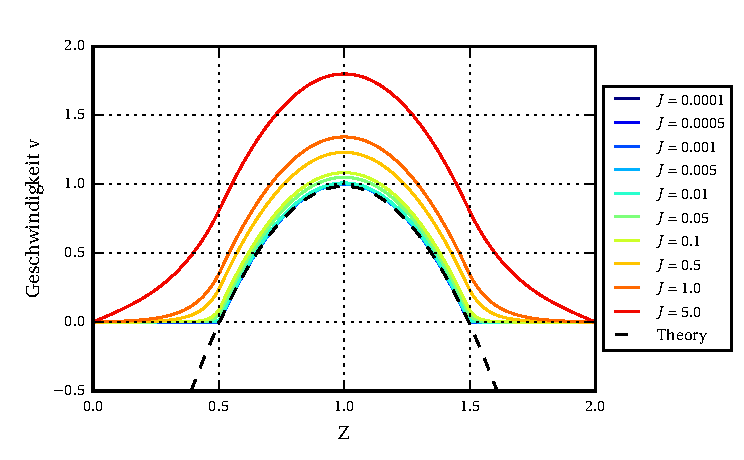
\includegraphics{gfx/immersed_boundary/poiseuille_flow/2_vp/vp_profile.pdf}  \caption{\label{fig:vp_flow}
    Velocity profile of the numerical solution with variable $J$ and $\Rey = 500$.}
\end{figure}

Furthermore


-a slight offset is introduced into the velocity profile (rest diskussion)

In the masked area of the volume we can see an exponential decrease of the total velocity.(erklärung diskussion)

2.For an error estimation, the relative $l_2$-error was computed.

The results for the 2nd order scheme are shown in figure \ref{fig:vp_error}.

\begin{figure}[!t]
  \centering
  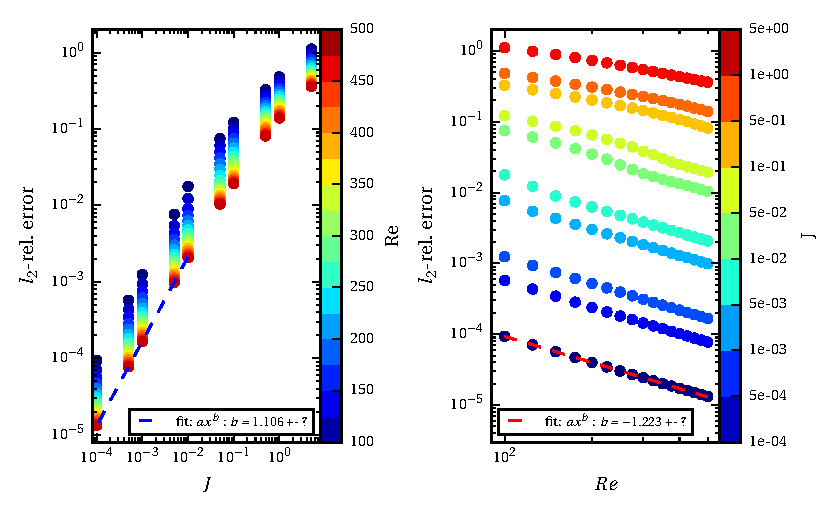
\includegraphics{gfx/immersed_boundary/poiseuille_flow/2_vp/vp_error.pdf}\label{fig:vp_error}
  \caption{Relative $l_2$-error for variable damping rate $\nu$ and reynolds-number $Re$.}
\end{figure}


3.The error decreases together with the damping rate from $1e-0$ to $1e-4$. For $nu<1e-3$ and a constant reynolds number we can observe an almost linear decrease in the logarithmic space,
this yiels a fit law of the form $ e = ax^b$. This shows that the error of this penalization method converges with first order in dependence of $\nu$.

4.Furthermore we can see a decrease of the error of one order with an increase in the reynolds number.

The results are shown in figure().

\begin{figure}[!t]
  \centering
  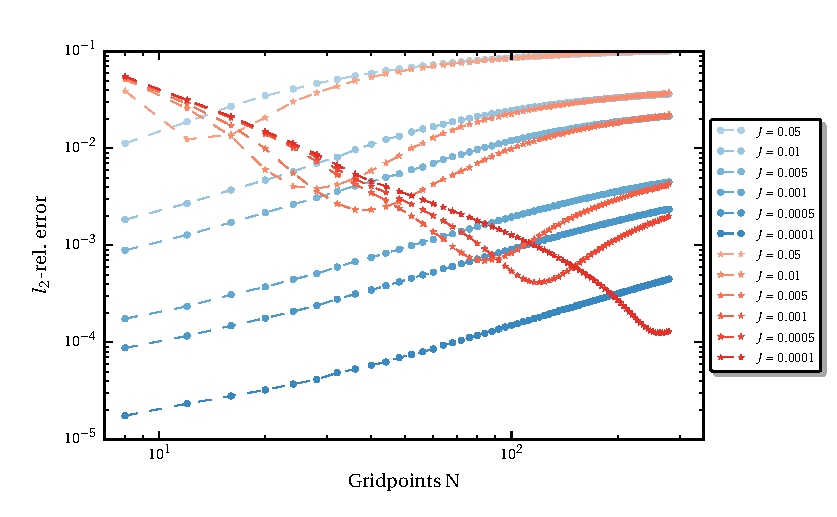
\includegraphics{gfx/immersed_boundary/poiseuille_flow/2_vp/vp_convergence.pdf}
  \caption{\label{fig:vp_conv}
      Relative $l_2$ error for variable damping rate $J$, for 2nd and 4th order finite difference schemes.}
\end{figure}
One can observe again that a decrease in $\nu$  yields a smaller error.
For the 2nd order scheme we can see that with an increase in the resolution, the error increases and finally converges against a constant value.
Even more confusing is the behaviour for the 4th order scheme.
With increasing resolution we can see a decrease into a local minimum, followed by an increase to the same error as the 2nd order scheme.

\clearpage

\subsection{Direct Forcing Method}
 the results are shown in figure X.

\clearpage


\section{Discussion}
\subsection{Poiseuille Flow}
\subsubsection{Test of the default setup}
For the finite difference scheme of 2nd order, the error behaves not as assumed.
Instead of the decline one would expect with the decrease of the resolution, the  error is nearly constant.
This behaviour can be explained due to the lack of complexity of the test case.
 As the theoretical solution is a polynom of 2nd order
no higher order terms will occur in the numerical solution, hence the
 2nd order scheme is capable of a perfect approximation, independent of the
grid resolution. The remaining error terms, are of the order $10e^{-8}$,
 which is extremly small and occur due to the floating point round off.
With this in mind the behavior of the 4th-order scheme is even more unexpected.
We see a linear decrease of the error on the log scale.
The result of a power law fit yields a convergence rate of 2nd order.
Furthermore the error is much larger compared to the 2nd order scheme,
 there is a decrease from $10e^{-2}$ to $10e^{-5}$.
The test case reveals that an error exists in the default implementation of the boundarie conditions.
An explanation can be given with comparison of the theoretical solution. The laplace operator is given by
 $ \nu \pdn[^2 v_x]{x^2} = 2A = \frac{1}{\nu}\pdn[p]{x}$
Using the mirroring method creates a discontinuous function at the boundaries, since the laplace operator changes the sign.
When using the 2nd order method the tree-point-stencil evaluates to the correct value $\pdn[^2 v_x]{x^2} = 1$.
The five-point-stencil of the 4th orderer scheme evaluates to $\pdn[^2 v_x]{x^2} = 1$, since it uses one point behind the boundary.
As a result the discontinuity creates an error in the higher order scheme.\\
For this testcase the 2nd order method yields better results, however we
have to keep in mind that the testcase yields a polynomial solution,
it is not clear how the results will end up for a complex testcase.
Furthermore in this testcase the boundaries have a large impact since the pressure gradient is parallel to wall,
his is not the case in general.
One possibility to avoid this error, would be to use an asymmetrich stencil, this approach is discussed in section ().

\subsubsection{Test of the Volume Penalization Method}
1.Since the damping can not fullfill the exact boundarie conditions, a slight offset is introduced into the velocity profile\\

2.
which leads to an offset in the solution.
Since for the steady state

\begin{align}
 \nu v &= D \frac{\partial^2 v_x}{\partial z^2}  \Rightarrow  v_x = A e^{\sqrt{\frac{\nu}{D}}v_x}
\end{align}

where A is given by the offset $v(h_1)$.\\

3.The decrease for $nu>=1e-3$ can be explained by having a look at figure \ref{fig:vp_flow} again. Since the damping in the masking area is to
weak the flow sees the real boundaries of the fluid domains, which results in a stronger damping on the flow.
This is not the case for $nu<1e-3$ since the velocities reaches zero before reaching the boundarie.\\

4.Since the damping force is proportional to the velocity and therefore to the reynolds number, the offset on the channel walls remains constant.
Due to the larger velocity profile this results in an smaller relative $l_2$-error, whereas the absolute error will increase.

An explanation of this behaviour can by given by revising the theoretical solution and the finite difference stencils at the immersed boundary.

The error does not converge towards zero, which means there has to be some discrepancy to the theoretical solution.
For a constant $\nu$ there is an offset to the theoretical solution, which we allready saw in figure (REF).
Hence by increasing the resolution the numerical solution converges towards the wrong solution.
The error increases since for a lower resolution, the velocity profile is closer to the assumed theoretical for the 2nd order method.

\begin{align}
 \nu v &= D \frac{\partial^2 v_x}{\partial z^2}  \Rightarrow  v_x = A e^{\sqrt{\frac{\nu}{D}}v_x}
\end{align}
\begin{figure}%
    \centering
    \subfloat[label 1]{{
      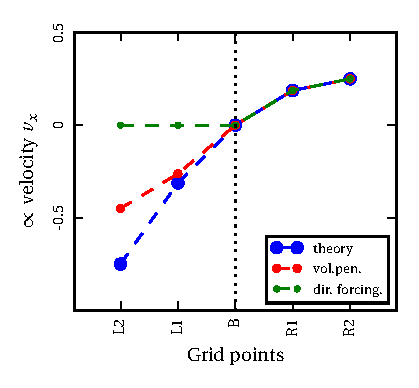
\includegraphics{gfx/immersed_boundary/poiseuille_flow/extra/stencil.pdf}\label{fig:mask_vp}
        }}%
    \qquad
    \subfloat[label 2]{{
      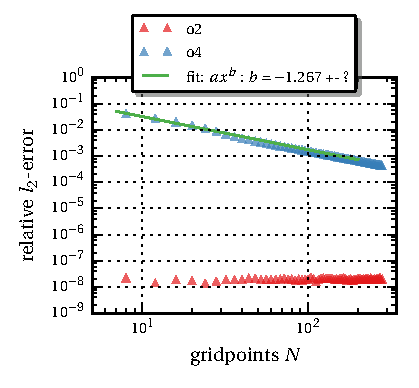
\includegraphics{gfx/immersed_boundary/poiseuille_flow/3_df/relative_l2error.pdf}\label{fig:mask_vp}
        }}%
    \label{fig:example}%
\end{figure}


The explanation for the 4th order convergence has again to do with the discretization error at the boundary.
Figure () shows schematically the velocity profiles for the volume penalizaton method compared to the theoretical.
Due to the different  profiles, the numerical evaluation of the laplace operator results
into different friction rates for the border point \textbf(B), but  also for the first next neighboor in the fluid domain \textbf(R1) when 4th order schemes are used.
For the 4th order scheme the laplace operator at the boundary evaluates to a slightly (CALCULATE) negative value), which means the friction at the boundary due to
viscosity is stronger. The result is a smaller velocity profile which when increasing the resolution starts to overlap best with the theoretical solution at the minimal error.
Finally when increasing the resolution further the error increases since the method converges towards the same resolution as the 2nd order scheme (IMAGE MAYBE?).
An attempt has been made to fit the numerical solution to a quadratic profile for the comparision to a theoretical solution but this didn't work due to blabla
(FIT IDEA NOT WORKING CONVERGENCE AGAINST HIGH RESOLUTION.

\subsection{Direct Forcing Method}
-We can see o4 not working reason is the same as we can se in figure n) , the laplacian is wrong caclulated at the point B.
As a results an error is induced at the boundaries of the domain.
The 2nd order scheme works perfectly as we compare it to the default implementation.


\subsection{Hagen-Poiseuille Flow}
\subsection{Taylor-Couette Flow}
\section{Summary}

\clearpage
\clearpage

\subsection{Hagen-Poiseuille Flow}

\subsubsection{Theoretical description}

In the previous testcase the channel walls were aligned parallel to the simulation grid, hence no further interpolation procedures
were necessary. In order to test the accuray of the interpolation methods, we now introduce a testcase with a curved geometry.
Furthermore we have the possibility to investigate the error of non-interpolating methods on curved surfaces.\\
The most simplest extension of the planar poiseuille flow, is the laminar flow through a pipe,
also referred to as Hagen-Poiseuille flow. The setup of the fluid domain is schematically shown in figure ().
We consider a flow in z-Direction where the total size of the simulation domain is set to $L_x = L_y = L$.
The immersed boundary is restricted by a wall at the radius $r_0=0.4L$ where r is defined as the distance from the pipe center $\vec{m} = (L/2, L/2)^T$.
The length $L_z$ can be chosen arbitrary due to the flow invariance in z direction.\\
\begin{figure}[!bp]
  \centering
  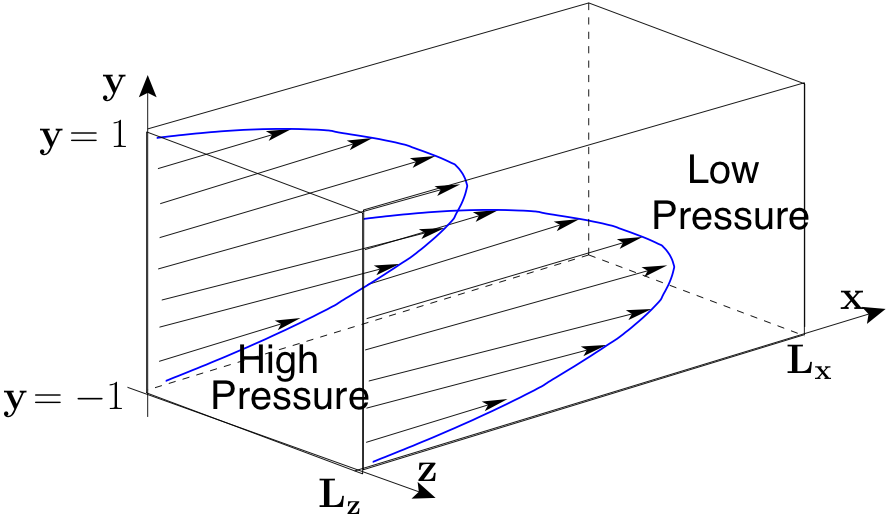
\includegraphics[width=0.8\textwidth]{gfx/immersed_boundary/val_volpen/poiseuilleflow.png}\label{b}
  \caption{Theoretical setup of the poiseuille-flow channel.}
\end{figure}
For an analytical solution of this problem we referr to [CITEFLUID].
Once again we can assume a steady state flow which implies $\partial v_z/\partial t = 0$. With the introduction of cylindrical coordinates $(r, \phi, x)$
and the assumption that the flow is independent of $\phi$ the equation of motion reduces to
\begin{align}
        0 &= - \frac{\partial p}{\partial x}  +  \frac{\nu}{r}\frac{\partial}{\partial r}\left(r\frac{\partial u}{\partial r}\right)
\end{align}
The solution is obtained by seperation of variables and integrating twice.
\begin{align}
    u &= \frac{r^2}{4\nu}\frac{\partial p}{\partial x} + A \ln r + B
\end{align}
By using the boundarie conditions $u(r_0) = 0$ and choose the same non-dimensionalization as in section (), with the expection of setting the length scale to $r_0$,
the velocity profile for the channel is given by
\begin{align}
    u &= \frac{r^2 - r_0^2}{4}\frac{\partial p}{\partial x}Re
\end{align}
Since $v_{max} \stackrel{!}{=} 1$ by definition, the pressure condition for the domain needs to be set to
\begin{align}
    \frac{\partial p}{\partial x} = -\frac{4 r_o^2}{Re}
\end{align}

\subsubsection{Grid Convergence Study}

For an error evaluation a grid convergence study was performed, for a constant reynolds number of $Re=100$.
The number of grid points was varied in the intervall $N\in[32, 256]$ with a stepsize of $\Delta N = 16$, furthermore a
simulation with a resolution of $N=512$ was carried out.\\
Since the maximum velocity of the channel is given by $v_{max}=1$, due to the choice of non-dimensionalization,
the sound speed was set to $c^2 = 100$ to fullfill the incompressibilty condition $Ma = v/c < 0.1$. \footnote{In order to exclude
any influence of choice of the sound speed on the resulting error, further simulations were carried out with a diffent $c^2$ and will be discussed}
With this choice the cfl-condition for the system is given by $\Delta t < \min(\Delta x^2 \cdot Re, \Delta x / 10)$.
The resulting timestep for the highest resolution is $\Delta t = 1e-4$.
With the above defined setup all methods introduced in section were tested, for 2nd and 4th order finite difference stencils.\\
For the penalization method the non-dimensionalized damping was set to $J=1e-4$.
It would be possible to choose a larger time step for the lower resolution cases, which means that in general
one would apply a smaller damping rate $J$ in a case of applicaton. To remain consistent in the error convergence, here $J$ and
therefore $\Delta t$ was not altered.\\
The results of the computation are shown from figure () to figure().
In figure (X) the relative $l_2$-error is shown for the volume penalization method with and without the volume fraction method
for 2nd and 4th order. The modified volume fraction method is not present since the computed error is almost identical to the default method,
such that the values overlap in the plot.

\begin{figure}[!pt]
  \centering
  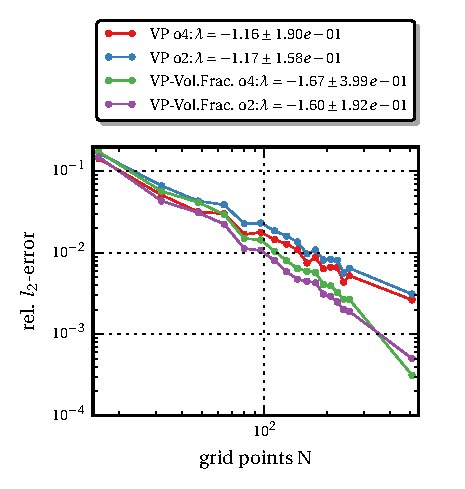
\includegraphics{gfx/immersed_boundary/hpflow/theo/vp.pdf}\label{fig:hpflow_vpgc_theo}
  \caption{blabla}
\end{figure}

\begin{figure}[!pb]
  \centering
  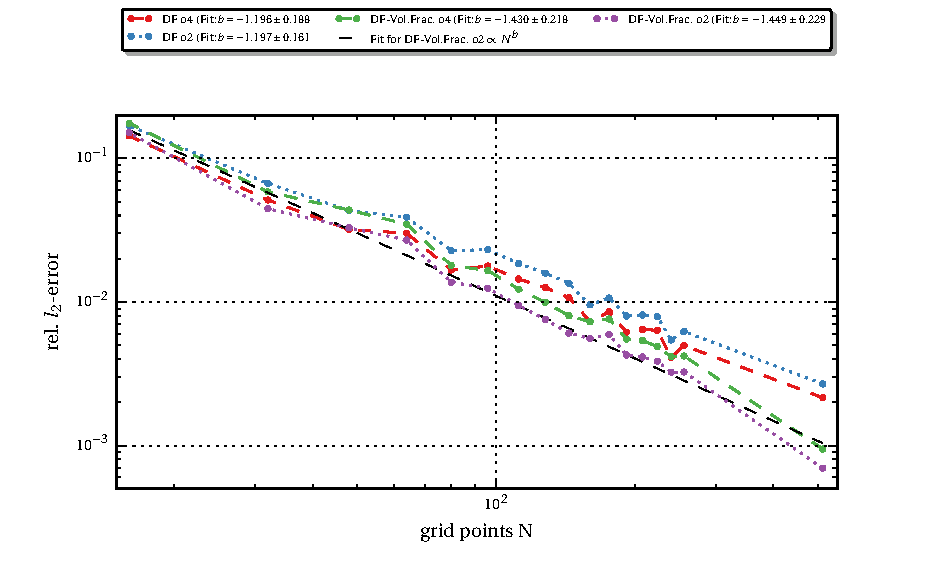
\includegraphics{gfx/immersed_boundary/hpflow/theo/df.pdf}\label{fig:hpflow_dfgc_theo}
  \caption{blabla}
\end{figure}


\begin{figure}[!pt]
  \centering
  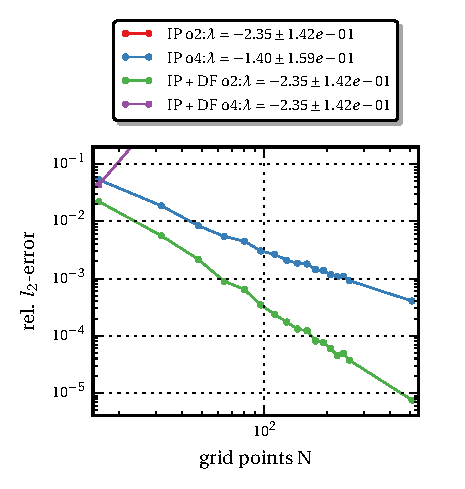
\includegraphics{gfx/immersed_boundary/hpflow/theo/ip.pdf}\label{fig:hpflow_ipgc_theo}
  \caption{blabla}
\end{figure}

\begin{figure}[!pb]
  \centering
  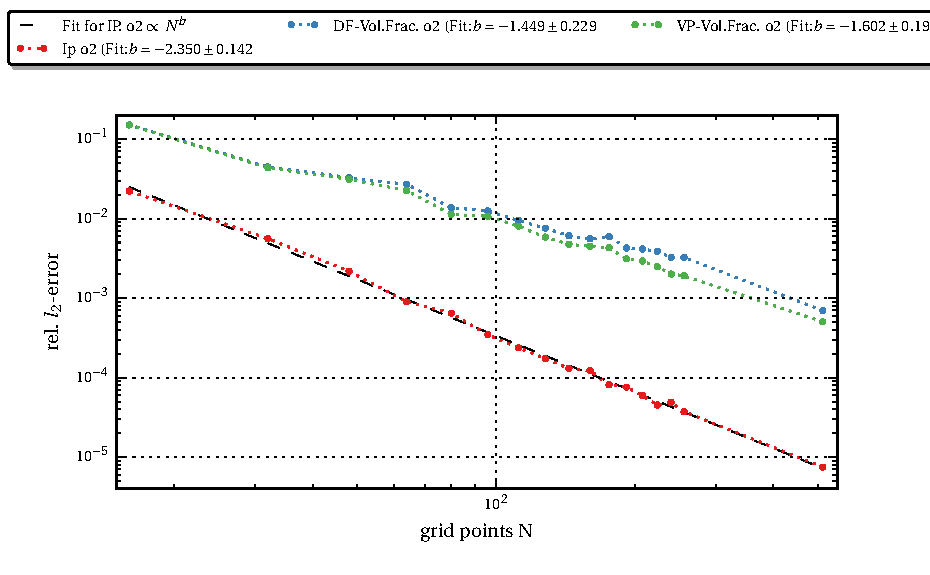
\includegraphics{gfx/immersed_boundary/hpflow/theo/all.pdf}\label{fig:hpflow_allgc_theo}
  \caption{blabla}
\end{figure}

\newpage

For all methods an approximately linear decrease  can be observed.
The error of volume penalizations methods decrease from the order $1e-1$ to $2e-3$, with
a convergence rate of order  $\epsilon \propto N^{\approx1.16}$
The volume fraction methods results in a slighty better convergence rate of $\approx 1.65$.
The overall error is smaller, due to the faster converge rates and of order $5e-4$ for the
highest resolution. For all methods the error is in the order of $1e-2$, above a resolution of 100 points.
The best results are achieved for the 2nd order volume fraction method, except for the highest resolution.\\
Figure () shows the error of the Direct Forcing method with and without the volume fraction method for 2nd
and 4th order. The error convergence is almost identical to the volume penalization method, when not using the volume
fraction method, of the order $\approx 1.2$. The convergence of the volume fraction methods is of order $\approx 1.45$
and therefore slighly weaker the for the volume penalization method.
As before the best error convergence is given by the volume fraction methond of 2nd order.\\
In Figure (X) we can see the error convergence of the interpolation schemes.
Here we used 2nd and 4th order schemes, furthermore we compare the interpolation with and without the
use of the direct forcing method.
The 4th order interpolation with direct forcing is not shown, since the resulting velocity fields are becoming
numerically unstable. The 4th order interpolation without DF also results into a larger error but in this case
the velocity field seems to be stable \footnote{This behaviour will be discussed in more detail in section ()}, the
convergence rate is of order $\approx 1.4$ and the error in the regime $1e-1$ to $4e-3$.
The best and furthermore identical results are achieved for the 2nd order interpolation with and without
use of the direct forcing method. The convergence rate is of order $\approx 2.35$ and the error
decreases from the order $2e-2$ to $1e-5$. The identy of these methods occurs due to the decoupling of the velocity fields
on the border ot the fluid domain. Since the interpolation stencil seperates the fluid and wall domain, the 2nd order
stencil doesn't see any points in the wall domain, therefore there is no difference in using the direct forcing method.\\
Finally figure () shows the previous methods with the best convergence rates in one plot.
In summary we can say that the overall converges rate of the interpolation method is of one order better
than the volume and direct forcing methods with volume fraction. Furthermore the relative error of the interpolation method ranges
between one and two order of magnitudes below all other methods, depending on the resolution.
The grid convergence study was than repeated once again in order to test the influence of the sound speed with $c^2 = 400$.
As a result it turned out that for all methods the difference in the relative $l_2$-error can be neglected, except
for the 4th order interpolation schemes, in this case the overall error grows. An exemplary plot which compares
the error can be found in Appendix in figure (). This behaviour indicates that when using the interpolation with 4th order
an error is induced which is proportional to $c^2\nabla \rho$.\\
As we allready could observe in section (), each immersed boundary method does not converge against the exact theoretical solution.
Therefore, for each method, a grid convergence study was peformed where the theoretical solution is given by a
high resolution solution of each method with $N=512$ points. This type of grid convergence study is often proposed
when no theoretical solution of the fluid problem can be achieved (SOURCE).
For this kind of grid convergence study the numerical setup is similar to the previous one with exeption of the resolution.
Here we use $N\in\{16, 32, 64, 128, 256\}$ for the number of grid points.
The problem occuring with other types of resolution is the position of grid points, which would not exactly overlap anymore with
the high resolution grid  of the theoretical solution of $N=512$.
An alternative would be to use interpolation methods for the exact positions, but the possible disadvantage with these method
would be an additional error resulting from the interpolation scheme.\\
The results of the error analysis are shown in figure () (a), exemplarly for the volume penalization, direct forcing  methods with volume fraction
and the interpolation method.

\begin{figure}[!pb]
  \centering
  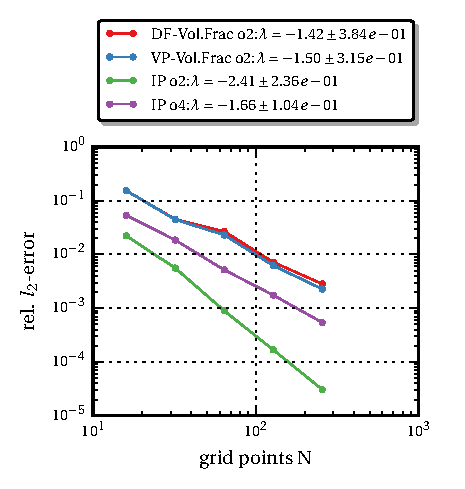
\includegraphics{gfx/immersed_boundary/hpflow/hd/all.pdf}\label{fig:hpflow_allgc_theo}
  \caption{blabla}
\end{figure}

The convergence rate of the volume penalization method and direct forcing method are of order $\approx 1.44$ and $\approx 1.6$.
Since the finite difference methods are of 2nd order, one would expect a similar decrease in the error.
However we can explain this behaviour by having a look at the velocity profile substracted from the theoretical solution.
Figure () (b) shows this exemplarly for the direct forcing volume fraction method. It can be noted that
the error vanishes in the middle section of the fluid error whereas the largest differences occur at the fluid domain border.
Therefore we propose that the bad convergence is caused by different approximations of the wall region for different resolutions.
Since the boundary is not mimiced exactly but approximated by the nearest neighboor points in the wall domain, the actual position
of the boundary is dependent of the resolution.\\
The interpolation method of 4th order converges with a rate of $\approx 1.4$ order. It is therefore even worse than the volume penalization and
direct forcing method, altough the overall error is smaller for lower resolutions. Again one possible explanation would be the different rasterization
of the domain border, which does not affect the velocity profiles due to the interpolation but the coupling of the pressure.\\
The 2nd order interpolation method converges is of order $\approx 2.35$, which is better than the expected order of two.
The fluid domain is interpolated at the same positions and since no pressure coupling over the fluid wall occurs the induced error is small.


\subsubsection{Long-Term Simulations}

In Order to test the  numerical stability, additionally a long-term simulation was performed for each IBM.
Again a Reynolds number of $Re=100$ was chosen, with a fixed resolution of $N=96$ grid points.


\begin{figure}[!pt]
  \centering
  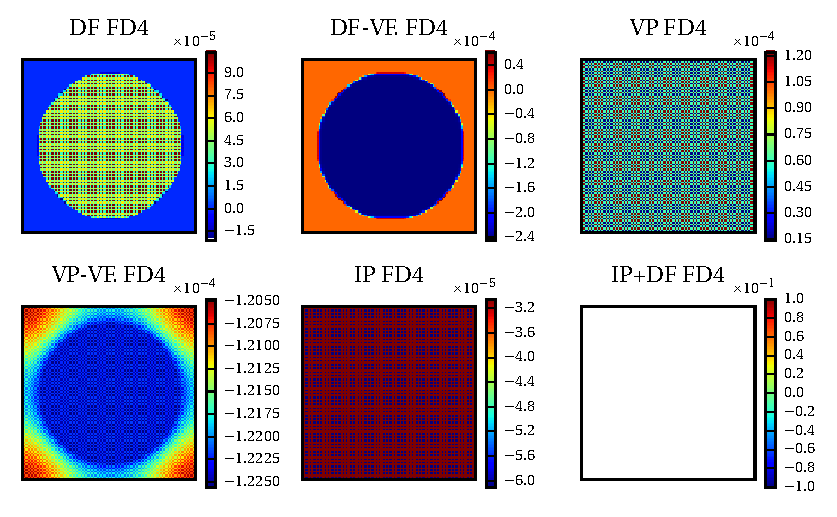
\includegraphics{gfx/immersed_boundary/hpflow/long/rho.pdf}\label{fig:hpflow_allgc_theo}
  \caption{blabla}
\end{figure}

\newpage

\begin{figure}[!pb]
  \centering
  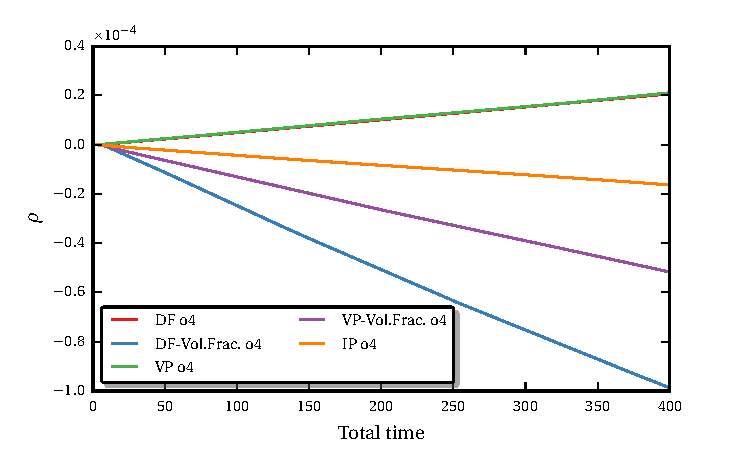
\includegraphics{gfx/immersed_boundary/hpflow/long/ts.pdf}\label{fig:hpflow_allgc_theo}
  \caption{blabla}
\end{figure}

\clearpage


\subsection{Taylor-Couette Flow}

\subsubsection{Theoretical description}
\begin{figure}[!b]
  \centering
  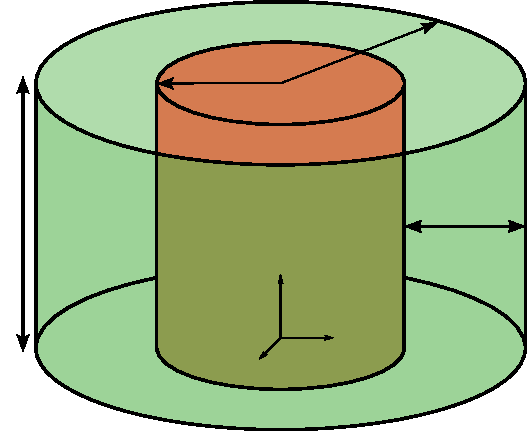
\includegraphics[width=0.3\textwidth]{gfx/immersed_boundary/tcflow/tcsystem.pdf}\label{fig:tcflow_system}
  \caption{Taylor Couette System with the inner and outer cylinder radius $R_1$ and $R_2$, and the rotation rates $\Omega_1$ and $\Omega_2$}
\end{figure}

As a last testcase for grid convergence studies we want to introduce the taylor-couette system.
The setup is exemplarly shown in figure (). It contains of two coaxial in z-direction oriented cylinders
with different radii $R_i$ and rotation rates $\Omega_i$. The fluid domain is given by the gap between the cylinders and
periodic in z-direction.\\
In dependency of the different domain paratemers different flow regimes can occur, criteria ...\\
We examine radial couette flow where the outter cylinder does not rotate ...\\
In constrast to the previously examined testcases this system provides different characteristics
of the flow regime at the fluid domain border. The flow along the borders is not orthogonal to the curvature of
the boundary like in the poiseuille flows we investigated before. Furthermore  new boundary
conditions are introduced, to be more precisely the Dirichlet condition is now given by $|\vec{v}(\vec{r})|_{r_i} | = |\Omega_i \times \vec{r}|$.
To begin with we want to examine the flow where the outer cyinder is not rotating, that is $\Omega_2 = 0$.
In literature this system is usually referred to as circular coutte flow (CCF) (CITE). Furthermore we want to investigate the flow regime
below the critical instability which means that $v_z=0$. In cylindrical coordinates the problem can be reduced to a two-dimensianol coordinate system with
the coordinates $(r, \phi)$, given by the coordinate transformations $x=r\cos(\phi), y = r\sin(\phi)$.
For the non-dimensionalization we choose the default convention (CITE) $x^*=x/(R_2 - R_1)$, $v^*=v/(R_1\Omega_1)$, $t^*=tR_1\Omega_1/(R_2-R_1)$ and $\rho^*=\rho$.
The flow is then characterized by the Reynolds number $Re = \frac{\Omega R_1d}{\nu}$. With this convention the equations of motion for the steady state are given by ()
\begin{align}
    -\frac{u^2_\phi}{r} = - \frac{\partial p}{\partial r}, 0 = \frac{1}{Re}\frac{\partial}{\partial r}\left(\frac{1}{r}\frac{\partial}{\partial r}(r u_\phi)\right)
\end{align}
Integrating the equations twice leads to the solution (CITE)
\begin{align}
    u_\phi = Ar + \frac{B}{r}
\end{align}
with
\begin{align}
    A = \frac{-\Omega_1R_1^2}{R^2_2 - R^2_1} ; B = \frac{\Omega_1R^2_1 R^2_2}{R^2_2 - R^2_1}
\end{align}

\subsubsection{Grid Convergence Study}

For the grid convergence study a reynolds number of $Re=50$  similar like in () was chosen in order to make sure the flow regime
is below the critical instability. With this exception all other parameters where kept the same like in section ().
The results of the computation are shown from figure () to figure ().

-


\newpage
\begin{figure}[!pt]
  \centering
  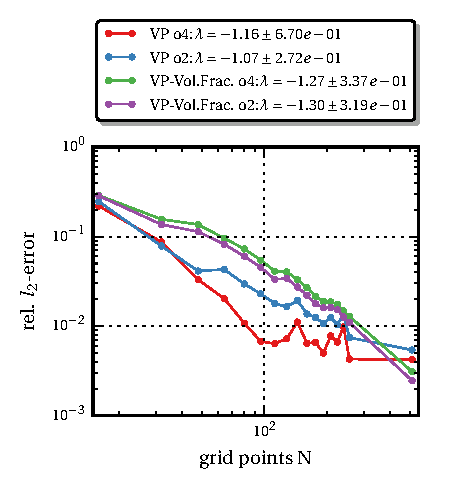
\includegraphics{gfx/immersed_boundary/tcflow/theo/vp.pdf}\label{fig:hpflow_vpgc_theo}
  \caption{blabla}
\end{figure}

\begin{figure}[!pb]
  \centering
  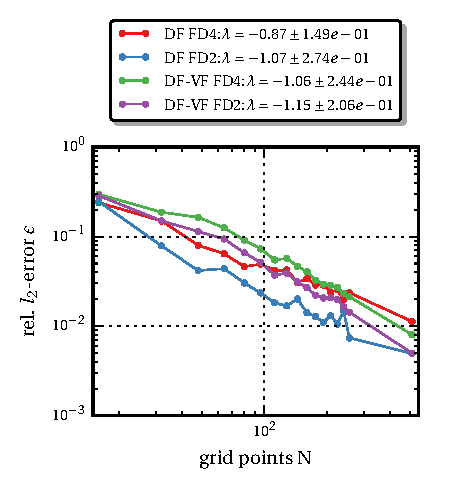
\includegraphics{gfx/immersed_boundary/tcflow/theo/df.pdf}\label{fig:hpflow_dfgc_theo}
  \caption{blabla}
\end{figure}


\begin{figure}[!pt]
  \centering
  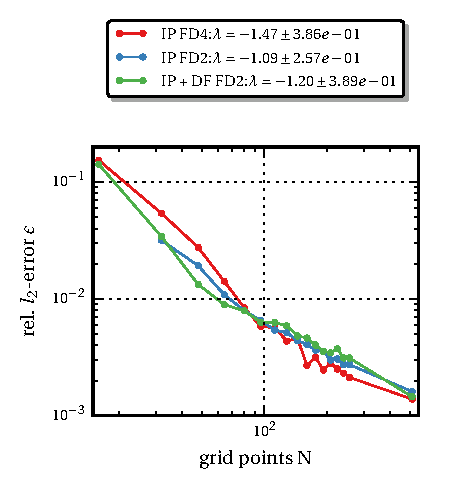
\includegraphics{gfx/immersed_boundary/tcflow/theo/ip.pdf}\label{fig:hpflow_ipgc_theo}
  \caption{blabla}
\end{figure}

\begin{figure}[!pb]
  \centering
  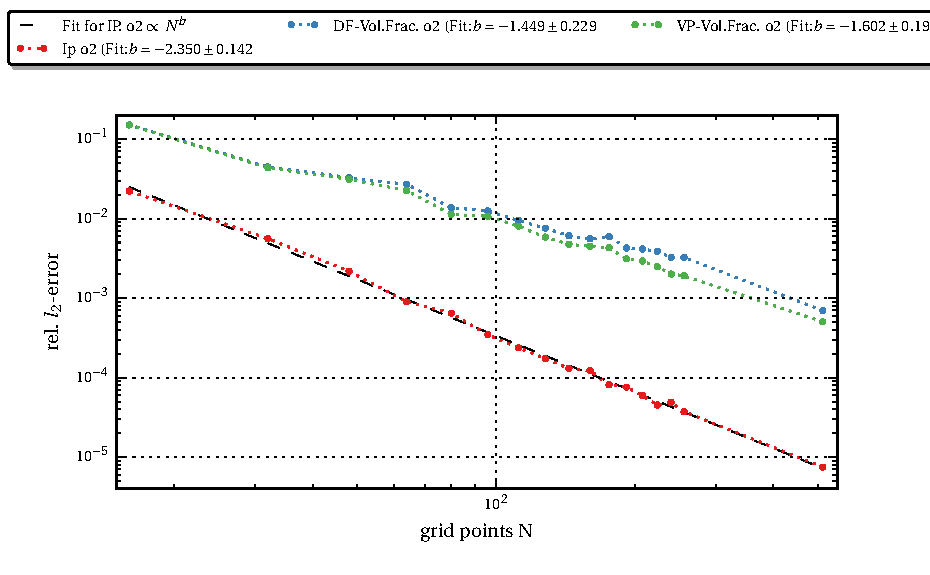
\includegraphics{gfx/immersed_boundary/hpflow/theo/all.pdf}\label{fig:hpflow_allgc_theo}
  \caption{blabla}
\end{figure}

\newpage



